\appendix
\chapter{Appendix}

\section{\texorpdfstring{A brief note on the tree $H_{C,1}$}{A brief note on the tree HC1}}
\label{appx:x_plus_1_variant}
A special case of Collatz trees is the graph $H_{C,1}$ -- the $x+1$ variant of $H_C$. In this case, any sequence of successive nodes along the path from $v_n$ down to $v_1$ is strictly monotonically increasing. If we run reverse to the edge direction (towards the root), then of course the node sequence is strictly monotonically decreasing. Figure~\ref{fig:hc1} shows a portion of the graph $H_{C,1}$ starting at its root.

\begin{figure}[H]
	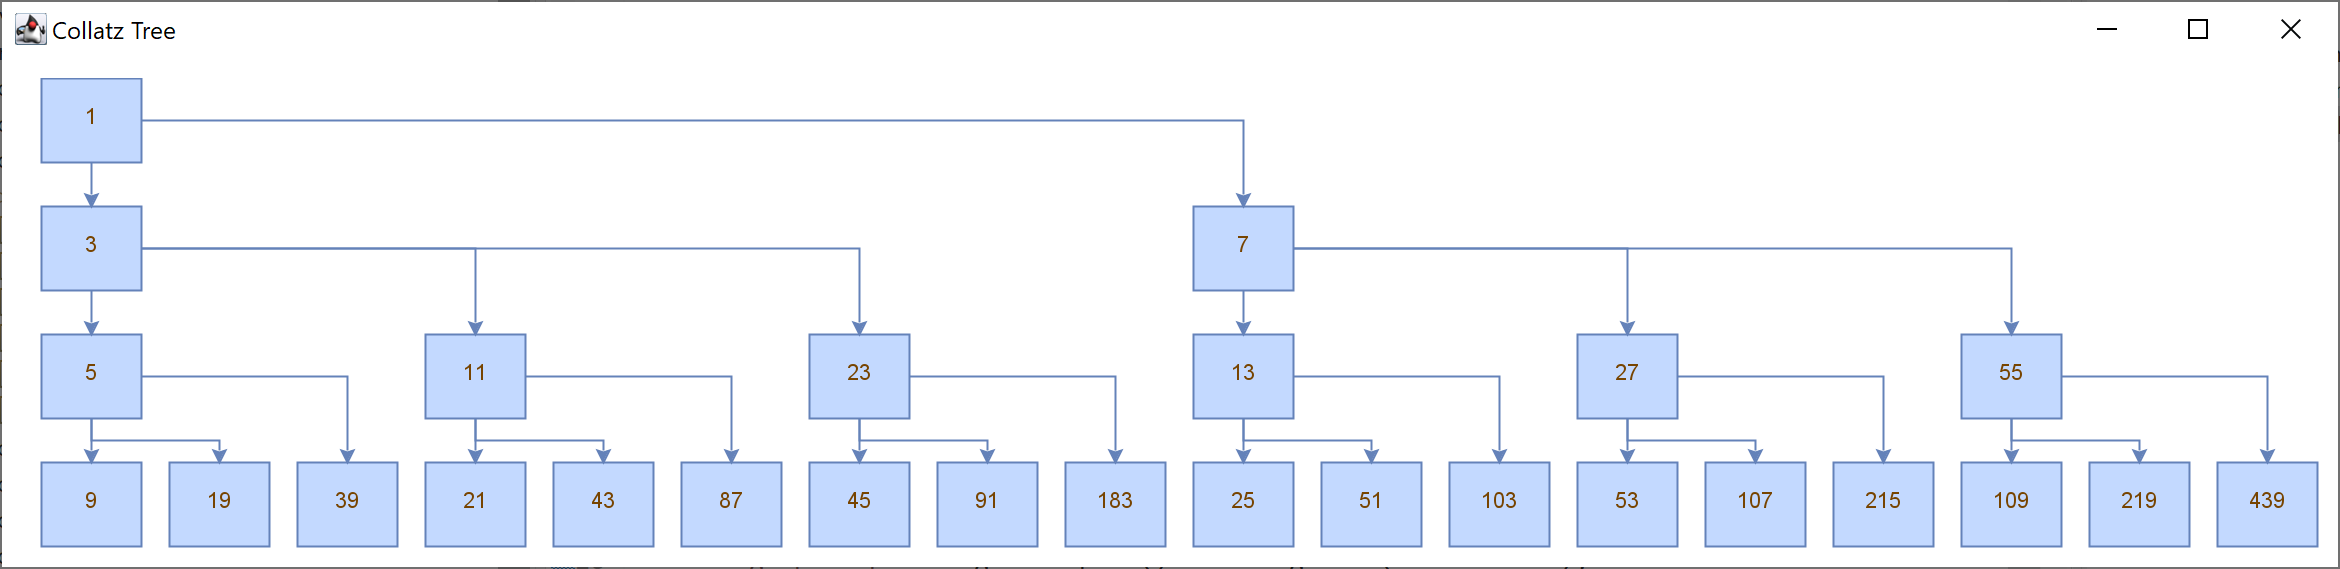
\includegraphics[width=1.00\textwidth]{figures/h_c1.png}
	\caption{Section of the graph $H_{C,1}$ starting at its root (without branches that reflect a subsequence containing the trivial cycle)}
	\label{fig:hc1}
\end{figure}

\section{\texorpdfstring{Algorithm for pruning binary trees $T_{\ge j}$}{Algorithm for pruning binary trees Tj}}
\label{appx:pruning}
Binary trees as introduced in chapter~\ref{ch:binary_tree} inspired by Kleinnijenhuis~\cite{Ref_Kleinnijenhuis_2020a}, \cite{Ref_Kleinnijenhuis_2020b} can iteratively be pruned (the way Kleinnijenhuis originally invented it). Listing~\ref{lst:pruning} implements this pruning algorithm.

\begin{listing}[H]
	\begin{minted}[bgcolor=bg, linenos, framesep=2mm, mathescape, breaklines, tabsize=2]{python}
def shrinkRoot(self):
	self.root = self.root.successors[0]
	self.root.predecessor = None

def prune(self):
	self.shrinkRoot()
	new_prunables = []
	for node in self.prunable_nodes:
		if node.predecessor is not None:
			if len(node.successors) > 1 and len(node.predecessor.successors) > 1:
				node.predecessor.successors[1].successors.append(node.successors[1])
				node.predecessor.successors[1].successors.reverse()
				node.successors[1].predecessor = node.predecessor.successors[1]
				node.successors[1].prunable = True
				new_prunables.append(node.successors[1])
			node.predecessor.successors.remove(node)
			node.predecessor = None
			self.labels.remove(node.label)
	self.prunable_nodes = new_prunables
	return self
	\end{minted}
	\caption{Python function for pruning a binary tree $T_{\ge j}$ \cite{Ref_Sultanow_Github}}
	\label{lst:pruning}
\end{listing}

Listing~\ref{lst:pruning} is only intended to illustrate the pruning algorithm in a simplifying manner. To run pruning on trees with arbitary large numbers, we refer to the professional Python API by Koch \cite{Ref_Koch_Github}.

\section{\texorpdfstring{The sum of reciprocated vertices depending only on $v_1$}{Sum of reciprocated vertices depending only on v1}}
\label{appx:sum_reciprocal_vertices}
One condition deduced from theorem~\ref{theo:1} is the product condition~\ref{eq:condition_max}, which specifies the validity of the cycle-alpha's upper limit. This condition requires the sum $\nicefrac{1}{kv_1}+\nicefrac{1}{kv_2}+\nicefrac{1}{kv_3}+\ldots$ to be limited. In order to formulate this sum independently from the successive vertices $v_2,v_3,\ldots$, we substitute these as follows:

\begin{flalign}
v_1&=v_1\notag\\
v_2&=\frac{kv_1+1}{2^{\alpha_1}}\notag\\
v_3&=\frac{k^2v_1+k+2^{\alpha_1}}{2^{\alpha_1+\alpha_2}}\notag\\
v_4&=\frac{k^3v_1+k^2+k\cdot2^{\alpha_1}+2^{\alpha_1+\alpha_2}}{2^{\alpha_1+\alpha_2+\alpha_3}}\label{eq:sum_v_4}\\
\vdots\notag\\
v_{n+1}&=\frac{k^nv_1+\sum_{j=1}^{n}k^{j-1}2^{\alpha_1+\ldots+\alpha_n-\sum_{l>n-j}\alpha_l}}{2^{\alpha_1+\ldots+\alpha_n}}\label{eq:sum_v_n_plus_1}
\end{flalign}

The sum of the reciprocated vertices can be expressed as a term that depends from $v_1$ and from the number of contracted edges, id est the number of dvisions by two, between two successive vertices $\alpha_1,\alpha_2,\alpha_3,\ldots$: 
\begin{equation*}
\sum_{i=1}^{n+1}\frac{1}{kv_i}=\frac{1}{k}\left(\frac{1}{v_1}+\sum_{i=1}^{n}\frac{1}{v_{i+1}}\right)=\frac{1}{k}\left(\frac{1}{v_1}+\sum_{i=1}^{n}\frac{2^{\alpha_1+\ldots+\alpha_i}}{k^iv_1+\sum_{j=1}^{i}k^{j-1}2^{\alpha_1+\ldots+\alpha_n-\sum_{l>i-j}\alpha_l}}\right)
\end{equation*}

\section{\texorpdfstring{The product of reciprocated vertices incremented by one}{The product of reciprocated vertices incremented by one}}
\label{appx:product_formula_depending_v1}
In a similar way to deduce the sum of reciprocated vertices depending only on $v_1$ as performed in \ref{appx:sum_reciprocal_vertices}, we evolve the product formula depending only on $v_1$:
\begin{flalign}
\prod_{i=1}^{n+1}\left(1+\frac{1}{kv_i}\right)&=1+\frac{2^{\alpha_1+\ldots+\alpha_n}+k\cdot2^{\alpha_1+\ldots+\alpha_{n-1}}+\ldots+k^{n-1}\cdot2^{\alpha_1}+k^n}{k^{n+1}v_1}\label{eq:prod_sum_v_n_plus_1}\\
&=1+\frac{2^{\alpha_1+\ldots+\alpha_n}+k\cdot\sum_{j=1}^{i}k^{j-1}2^{\alpha_1+\ldots+\alpha_n-\sum_{l>i-j}\alpha_l}}{k^{n+1}v_1}\label{eq:prod_sum_v_n_plus_1_inserted}\\
&=1+\frac{2^{\alpha_1+\ldots+\alpha_n}+k\cdot\left(v_{n+1}\cdot2^{\alpha_1+\ldots+\alpha_n}-k^nv_1\right)}{k^{n+1}v_1}\notag\\
&=\frac{2^{\alpha_1+\ldots+\alpha_n}\left(1+kv_{n+1}\right)}{k^{n+1}v_1}\label{eq:prod_sum_v_n_plus_1_simplified}
\end{flalign}
We inserted the sum used in equation~\ref{eq:sum_v_n_plus_1} into the above-given equation~\ref{eq:prod_sum_v_n_plus_1} and then obtained equation~\ref{eq:prod_sum_v_n_plus_1_inserted}. Let us divide this product by the last factor and consider the product in the condition for cycle-alpha's upper limit, which iterates to $n$ instead of $n+1$:

\begin{equation}
\label{eq:prod_sum_v_n_simplified}
\prod_{i=1}^{n}\left(1+\frac{1}{kv_i}\right)=\frac{\prod_{i=1}^{n+1}\left(1+\frac{1}{kv_i}\right)}{\frac{kv_{n+1}+1}{kv_{n+1}}}=\frac{2^{\alpha_1+\ldots+\alpha_n}\cancel{\left(1+kv_{n+1}\right)}kv_{n+1}}{k^{n+1}v_1\cancel{\left(kv_{n+1}+1\right)}}=\frac{2^{\alpha_1+\ldots+\alpha_n}v_{n+1}}{k^nv_1}
\end{equation}

The above-shown equation~\ref{eq:prod_sum_v_n_simplified} becomes simplified, when we replaced the numerator by equation~\ref{eq:prod_sum_v_n_plus_1_simplified}. The question which sequence maximizes its last member $v_{n+1}$ ties into the question: Which sequence maximizes the product? The product formula~\ref{eq:prod_sum_v_n_simplified} does not depend from all vertices $v_1,v_2,\ldots,v_n$, it depends only from $2^\alpha=2^{\alpha_1+\ldots+\alpha_n}$, from the first vertex $v_1$ and the final one $v_{n+1}$.

